% #################################################################################
%
% LaTeX Template LaTeX for Internoise 2019
%
%
% #################################################################################
\documentclass[a4paper,12pt]{article}


%% Pick the one corresponding to your system
%\usepackage[latin1]{inputenc}
%\usepackage[ansinew]{inputenc}
\usepackage[utf8x]{inputenc}
\usepackage[T1]{fontenc}
\usepackage{times}
\usepackage[colorlinks=true,linkcolor=black,citecolor=black,urlcolor=blue]{hyperref}
\usepackage{geometry}
\geometry{top=2cm,bottom=2cm,left=2.0cm,right=2.0cm}
\pagestyle{empty}

\usepackage{titlesec}
\titleformat{\section}
{\bfseries\uppercase}{\thesection.}{1em}{}
\titleformat{\subsection}
{\bfseries}{\thesection.\thesubsection.}{1em}{}
\renewcommand{\labelitemi}{\textendash}
\renewcommand{\labelitemii}{\textendash}

\usepackage{graphicx} % used to insert the figure
\usepackage{multirow} % used for the table
\usepackage[font=it]{caption}
\usepackage{cite}
\usepackage{breakurl}
\usepackage{indentfirst}
\usepackage{amsmath, amssymb, amsfonts, bm}
\usepackage{txfonts}
\usepackage{enumitem}
\usepackage{xcolor}

\hyphenpenalty=10000
\setlength{\emergencystretch}{3em}

\columnsep 1cm
\setlength{\parindent}{0.5cm}

\titlespacing*{\subsection}{0pt}{1.5em}{0.2em}


\renewcommand\eqref[1]{Equation~\ref{#1}}

\renewcommand{\thesection}{\arabic{section}}
\renewcommand{\thesubsection}{\arabic{subsection}}


\renewcommand{\refname}{6. \hspace{3mm} REFERENCES} 
\setlength{\footnotesep}{12pt}

\begin{document}

\begin{center}
	
\includegraphics[width=38.8mm, height=20.6mm]{logo2020.png}
\end{center}
\vskip.5cm

\begin{flushleft}
\fontsize{16}{20}\selectfont\bfseries

\color{black}Compressed Air Leakage Detection Using Acoustic Emissions with
Neural Networks
\end{flushleft}
\vskip1cm

\renewcommand\baselinestretch{1}
\begin{flushleft}

Given name Family Name1\footnote{mail1@example.com}\\
Institution\\
Full address\\

\vskip.5cm
Given name Family Name2\footnote{mail2@example.com}\\
Institution\\
Full address\\

\vskip.5cm
Given name Family Name2\footnote{mail2@example.com}\\
Institution\\
Full address\\

\vskip.5cm
Jakob Kirner\footnote{jakob.kirner@protonmail.com}\\
Technische Universität Ilmenau\\
Full address\\

\end{flushleft}

\textbf{\centerline{ABSTRACT}\\
Compressed air is utilized in many branches of industry and one of the most expensive energy sources of industrial plants. Therefore, efficient detection of air pressure leaks goes hand in hand with cost savings and increased  operational reliability. Some procedures of leakage detection for pressure lines are based upon the analysis of sound emissions. Such solutions detect specified ultrasonic emission patterns or, alternatively, personnel trained to hear the sounds are deployed for leakage detection.\\ In this paper, we evaluate the potential of using airborne sound emissions in the audible hearing range for the automated detection of compressed air leakage using artificial neural networks. Therefore, a novel dataset was created and published. It contains recordings from several microphones at different distances of adjustable leakage from a pneumatic contraption with different pressure levels. Additionally, industrial background noises were applied at different levels to simulate real-world sound environments. Using this dataset, a deep neural network was trained for leakage detection. The results show that leakage detection by means of airborne sound in the audible range using machine learning techniques is possible, and is a promising contactless and automatic detection method.}


\section{Introduction}

The use of compressed air (CA) as a source of energy is part of many branches of industry. In the field of mobility, a large number of pneumatic systems are used in commercial vehicles and passenger transport. As in manufacturing, undesired gas leakage due to leaks and leaks is a frequent error pattern: Exposure of CA carriers in the area of the chassis as well as vibration make regular inspections unavoidable.  Reliable maintenance methods for gas carriers ensure safety and energy and thus cost savings \cite{Radgen.2001}. 	
Some leakage measurement methods are based on the measurement of sound emissions.  In a given case, turbulent leakage of CA produces clear emission patterns that spread both through the air and through adjacent bodies. For the airborne sound based detection of leaks, localisation by ultrasound is a common method, whereby the detection process must take place in the immediate vicinity of the gas carrier \cite{Chen.2007}. 
In order to avoid the distance problem of ultrasonic technologies for leak detection, this paper investigates the possibility of airborne sound based leak detection in the auditory range (20 Hz - 20 kHz). 	
In addition, the integration of a machine learning system into the detection process  creates new perspectives: A deep neural network (DNN) is used, the configuration of which has already proven itself in the detection of anomalies in components \cite{EstefaniaCanoJohannesNowakandSaschaGrollmisch.}. This network is trained to detect the sound signatures of CA leaks in different scenarios.

\section{Basics}
\subsection{The physics of leakages}

A real gas pumping system can never be absolutely tight. DIN EN 1779 lists the so-called leakage rate as a measure of the urgency of a maintenance measure. The following applies: From $q_L > >10^{-2}$ mbarL/s a leakage is classified as "turbulent" \cite{1779}. On a physical level, the pressure difference between the pipeline and the environment is so high that turbulence forms when the pipeline gas escapes. Only the occurrence of turbulence allows the leakage to be detected acoustically \cite{Genuit.2010}. The exhaust jet can be regarded as an acoustic source in the form of a quadrupole emitter \cite{Zeller.2018}, which can also be recorded well from lateral microphone positions.

\subsection{Machine Learning}
The term machine learning (ML) refers to a variety of different system architectures and computational models that have a wide range of applications \cite{FHG.2018}. ML systems can be classified into the categories supervised, semi-supervised and unsupervised according to the type of training data initially supplied. The different degrees of supervision or monitoring have the following meaning: In supervised procedures, annotated data and an expected result are given. In the unsupervised procedure, the ML system extracts its own characteristics from a data record. If a result is queried, the system can show correlations with specific input data. The semi-supervised procedure is the hybrid form \cite{Bishop.2009}.
Deep neural networks (DNN) analyze input data and compare them with given or learned characteristics \cite{FHG.2018}. The DNN thus trained, together with the acquired knowledge, can in turn be applied to other data sets of the same type. The prerequisite is a sufficiently large data set. 
DNNs have the advantage that they can learn and map non-linear processes very well without being given mathematical rules \cite{ZHANG.2004}. This in turn means that a DNN-supported sensor system has to rely on less domain and expert knowledge than other ML systems \cite{FHG.2018}. If a DNN is to be trained for the purpose of state classification, a corresponding acquisition of factual prior knowledge or a corresponding annotation is indispensable \cite{ltu.luscha}. 

\section{Setup}

The test object is a Festo Didactic System, which consists of a tool table with a rail field that can be freely equipped with various pneumatic elements. By means of this modular system, a simple pneumatic circuit is to be implemented. The use-cases of a a leaking connection point and worn tubing is simulated. Here the leakage noises are generated by a combination of a choke vent (CV1) with another choke vent (CV2) or folded tubing. CV1 regulates the airflow by turning a knurled screw that generates variable flow resistance. 

\subsection{Microphone setup}

For optimum recording of the leakage noise, microphones with an omnidirectional characteristic and sufficiently linear frequency response in the range 1 - 20 kHz is used (Earthworks M30). Eight microphones are paired to four fixed positions.  Two microphone positions with 6 cm and 60 cm are held by markings. The microphone is directed laterally towards the valve in order to obtain as much as possible of the sound field discussed in chapter 2.5 of the escaping free jet.

 \begin{minipage}{\textwidth}
  \begin{minipage}[b]{0.49\textwidth}
    \centering
    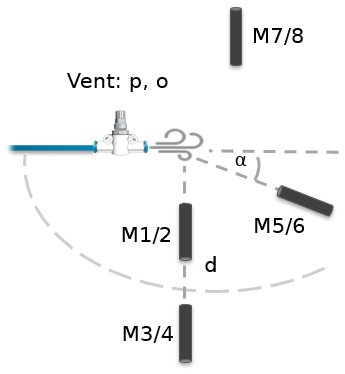
\includegraphics[width=55mm]{images/mic_positions_scheme.png}
    \captionof{figure}{A table beside a figure}
  \end{minipage}
  \hfill
  \begin{minipage}[b]{0.49\textwidth}
    \centering
    \begin{tabular}{ll}
    Microphones & Position\\
    \hline
    \textbf{M1/2} & 20 cm distance, 90° to leakage\\
    \textbf{M3/4}& 2 m distance, 90° to leakage\\
    \textbf{M5/6}& 20 cm distance, $\alpha < 30°$\\
    \textbf{M7/8}   & Ambient recording of whole room   
    \label{tab:mics}
    \end{tabular}
      \captionof{table}{A table beside a figure}
    \end{minipage}
  \end{minipage}

\subsection{Generating a two-class problem}

Fig. 1 illustrates the detection process: Leakage type and internal pressure of a pipe cause turbulences (1.), which are described in radiation characteristics as well as, depending on the frequency range under consideration an acoustic profile. The space between the transmitter and receiver also has an Numerous influencing variables that influence the measurement signal. Thus the direct For example, the distance between the sound source and microphone is decisivefor signal levels and runtime-dependent effects. In addition, in practice overlaps by ambient noise and spatial influences such as reflections and diffuse sound.

\begin{figure}[h]
	\centering
	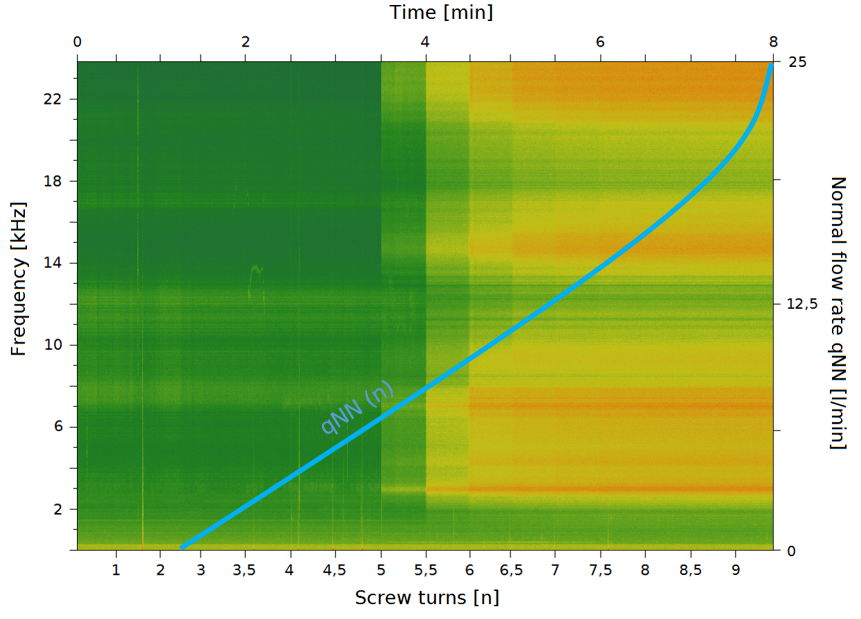
\includegraphics[width=88mm]{images/V_1_normi_qnn.png}
	\caption{Spectrogram of leakage noise from microfone position 1 with characteristic vent flow rate for 6 Bar}
	\label{fig:spec+qnn}
\end{figure}

The spectrogram in fig shows the recording of the leakage noise. The frequencies of the turbulently exiting air are plotted over time and the number of screw rotations. To increase visibility of the leakage sounds main features, gain is added. Recorded sound events are displayed relatively to the recording threshold level from green (low) via yellow (medium) to red (high). The knurled screw on valve two is now opened in $30s$ intervals by a fixed amount. For the interval $0 < n  3$ whole rotations are made. This action is based on consideration of the component characteristic curve (blue) from \ref{fig:spec+qnn}. From $n = 3$ half turns are made on the second screw to increase the accuracy. The resulting Recordings are later used as a reference for a leak-free environment.

If you now look at frequencies and levels, the following becomes apparent: In the range 0 < n < 5.0 the microphone does not register any periodically occurring signal. If the screw is turned up further from $n = 5$ to $n = 5.5$ on a level maximum in the range 3.1 kHz, 7.1  kHz in the range 9.2 kHz or 14.8 kHz and beyond the audible spectrum become visible. The increasing sound level at larger n is highlighted by red coloring. For increasing screw turns the volume around those frequency bands increases the peak levels of the prominent bands however are not influenced by the screw position. Thus the average values of the frequency bands remain constant. For the upcoming measurements a signal threshold of $n = 5$ is assumed. \ref{tab:mappingclasses} links the screw turns to the two conditions \textit{no leakage/OK} and \textit{leakage/nOK}.

\begin{table}[h]
    \centering
	\begin{tabular}{ | l | c | c | c | c | c | c | c | c | c | }
		\hline
		n $=$  & 0 & . . . & 3 & 3.5 & . . . & 5 & 5.5 & . . . & 9 \\ \hline
		Condition & $OK$ &   . . . & $OK$ & $OK$ & . . . & $OK$ & $nOK$ & . . . & $nOK$ \\ \hline
		\multicolumn{1}{c}{} & \multicolumn{3}{c}{\upbracefill}& \multicolumn{3}{c}{\upbracefill}& \multicolumn{3}{c}{\upbracefill}\\[-1ex]
		\multicolumn{1}{c}{} & \multicolumn{3}{c}{no leak} &\multicolumn{3}{c}{leak not detectable}&\multicolumn{3}{c}{leak detectable}
	\end{tabular}
	\caption{Mapping screw turns to binary classes.}
	\label{tab:mappingclasses}
\end{table}

\subsection{Measurement series}

\begin{table}[h]
    \begin{tabular}{lll}
    \centering
    Code       & Name      & Parameters/Description\\
    \hline
    \textbf{v} & Vanilla   & 6 Bar, choke vent, quiet lab\\ 
    \textbf{p} & Pressure  & 5 Bar, choke vent, quiet lab\\
    \textbf{o} & Opening   & 6 Bar, tubing, quiet lab\\     
    \textbf{w} & Workshop  & 6 Bar, choke vent, added aperiodic workshop ambient sounds\\
    \textbf{h} & Hydraulic & 6 Bar, choke vent, added periodic sound of screeching piston\\
    \label{series}
    \end{tabular}
\end{table}

\section{Results}

[...]
Visible in figure \ref{fig:meanfracc} 
- mean accuracy values of all experiments per microphone position
- arithmetic mean (black) and max deviation (grey)
- similar mean accuracy at similar distance 
- odd numbers (high gain) in microphone pairs have lower mean accuracy than even numbers (low gain)

\begin{figure}[h]
	\centering
	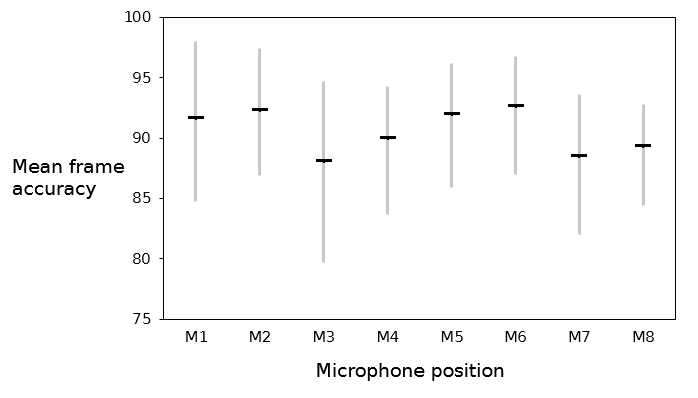
\includegraphics[width=88mm]{images/mean_frame_acc.png}
	\caption{Spectrogram of leakage noise from microfone position 1 with characteristic vent flow rate for 6 Bar}
	\label{fig:meanfracc}
\end{figure}

\iffalse


\begin{figure}[h]
	\centering
	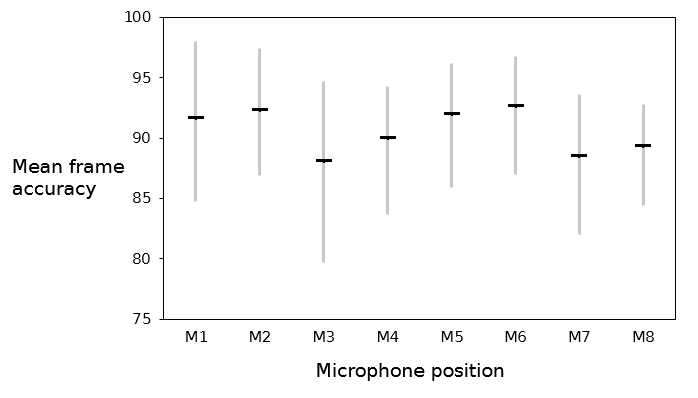
\includegraphics[width=88mm]{images/mean_frame_acc.png}
	\caption{Mean (frame) detection accuracy per microphone position (M)}
	\label{fig:mean_frame_acc}
\end{figure}




\begin{table}[h]
    \centering
    \begin{tabular}{lllllllll}
    & 1m    & 1l    & 2m    & 2l    & 3m    & 3l    & 4m    & 4l    \\
    \hline
    v  & 97,97 & 96,06 & 94,65 & 94,23 & 95,19 & 94,62 & 93,22 & 91,86 \\
    p  & 93,16 & 92,37 & 82,85 & 83,69 & 93,7  & 93,04 & 90,09 & 87    \\
    o  & 97,81 & 97,4  & 93,65 & 93,52 & 94,83 & 96,72 & 93,63 & 88,56 \\
    w  & 92,86 & 91,38 & 90,36 & 90,31 & 90,04 & 93,04 & 90,34 & 90,26 \\
    h  & 92,29 & 93,69 & 88,52 & 93,51 & 96,15 & 94,88 & 89,2  & 92,55 \\
    po & 93,54 & 93,51 & 91,76 & 90,96 & 93,18 & 94,46 & 90,52 & 92,8  \\
    oh & 86,17 & 92,01 & 79,68 & 90,92 & 90,8  & 89,55 & 82,09 & 89,27 \\
    ow & 86,81 & 87,86 & 85,29 & 85,4  & 87,77 & 90,61 & 85,65 & 84,37 \\
    ph & 84,7  & 86,93 & 86,35 & 87,06 & 85,93 & 86,96 & 81,97 & 87,27 \\
    \hline
    \caption{Mean frame accuracy for microphone positions}
	\label{tab:mappingclasses}
    \end{tabular}
\end{table}


\section{Experiment}
\section{Setup}
\section{Acknowledgement}




\subsection{Margin Settings}

\begin{itemize}
	\item The paper size is A4.
	\item Margin settings: Top (2.5 cm), Bottom (2.5 cm), Left (3.0 cm), Right (3.0 cm)
	\item The text should be justified from left to right.
	\item The first line of the paragraphs should be indented by 0.5 cm. 
\end{itemize}

\subsection{Paragraphs}

\begin{itemize}
	\item There should be one empty line between headings and subheadings.
	\item Major headings shall be numerically ordered as 1., 2., …., in bold font.
	\item Level 2 subheading should be 2.1, 2.2, ..., in bold font.
\end{itemize}

\subsection{Figures, Tables and Equations}
All figures, tables, equations, photos, graphs, etc., must be shown shortly after they are mentioned, placed at the centre of a page. \par 
The caption of figures and photos are put below the figures and photos in italic font ~\cite{andre18}(see Figure~\ref{fig:logo}).

\begin{figure}[!h]
	\centering
	
\includegraphics[width=88mm]{logo2020.png}
	\caption{Logo of Inter-Noise 2020}
	\label{fig:logo}
\end{figure}

The equations should be referenced as Equation 1, Equation 2, etc.
\eqref{eq} is an example.  

\begin{equation}
	\bar x= \frac{1}{N}\sum_ix_i
	\label{eq}
\end{equation}

The caption of tables should be placed just above the tables in italic font and the table number should be Table 1, Table 2, … like Table~\ref{tab:table1} below.

\begin{table}[h!]
  \begin{center}
    \caption{Example}  
    \label{tab:table1}
    \begin{tabular}{c c c} 
     \hline	
      \textbf{Value 1} & \textbf{Value 2} & \textbf{Value 3}\\
      \hline
      1 & 1.1 & a\\
      \hline	
      2 & 2.2 & b\\
      \hline	
    \end{tabular}
  \end{center}

\end{table}



\section{Important information}

\subsection{Submission of Manuscripts}

The manuscript should be submiited as a PDF file through the INTER-NOISE 2019 website
(\url{www.internoise2020.org}). \par
Before submitting the manuscript, you need to pay the registration fee and if you submit mutiple manuscripts, you need pay extra nominal charge for each manuscript.


\subsection{Conversion to PDF}

Before submission, you need to check your PDF file carefully to be sure that PDF conversion was
done properly and there is no error when the PDF file is opened. 
The following problems may occur.

\begin{itemize}
\item Symbols are missed.
\item Symbols are converted incorrectly, especially mathematical symbols.
\item Figures are missed.
\item Indentation is not correct.
\end{itemize}

The author is responsible for these problems and the manuscript will publish in the Congress Proceeding as it is received.

\section{Conclusions}
This is the conclusion section.

\fi

\section{Acknowledgements}
We gratefully acknowledge Lena Zentner and Dirk Wetzlich from FG Nachgiebige Systeme at Technische Universität Ilmenau for providing the central infrastructure for our experiments.



\bibliography{biblio} 
\bibliographystyle{ieeetr}





\end{document}


